\chapter{Introduction and Background Research}

% You can cite chapters by using '\ref{chapter1}', where the label must
% match that given in the 'label' command, as on the next line.
\label{chapter1}

% Sections and sub-sections can be declared using \section and \subsection.
% There is also a \subsubsection, but consider carefully if you really need
% so many layers of section structure.
\section{Introduction}
\label{chapter1:introduction}

Operating systems (OSes) are specialised, low level software that manages a computer's
resources and provides a common interface for programs. The most common operating
systems used by most consumers today include MacOS and Windows. Xv6 is an operating
system written by MIT for the purposes of teaching, which runs on the RISC-V architecture \cite{xv6:book}\cite{xv6:code}.
As it is meant to be a teaching OS, it has very barebones functionality,
which includes a command line shell and some basic user programs by default.

This project aims to extend Xv6 with some graphics functionality.


% Must provide evidence of a literature review. Use sections
% and subsections as they make sense for your project.
\section{Background research}
\subsection{Xv6}
As mentioned in Chapter \ref{chapter1:introduction}, Xv6 is a barebones OS used for teaching purposes developed by MIT.
Its features include:
\begin{itemize}
    \item Based on UNIX v6 (hence the v6 in Xv6)
    \item Written for 64 bit RISC-V architecture
    \item Multicore support with a round robin scheduler
    \item Runs on QEMU (qemu-system-riscv64)
\end{itemize}

\subsection{QEMU}
QEMU is an emulator that allows running a guest operating system that may run on
a different target hardware platform. In our case we will be running Xv6,
which runs on the RISC-V architecture, in QEMU for development and testing.


It also provides a way to debug the kernel through a GDB serial port, which greatly
eases development and testing as we can connect a graphical debugger to the kernel.


We will also be using its device emulation to emulate a VGA card on the PCI bus 
for our driver to communicate with to display graphics. It offers many options 
each with its own pros and cons ranging from a simple VGA device with a linear framebuffer
to cards with hardware acceleration. Additionally, QEMU also
provides a simulated display that can be viewed through a VNC client, so we can
see the graphics output of Xv6.

\subsection{VGA}
VGA (Video Graphics Array) has a well defined but complex hardware standard.
Although complex, there is an abundance of technical resources
\cite{vgamanual}
\cite{osdevvga}
\cite{freevga}
that can
assist in developing a VGA driver. In addition, QEMU can emulate a VGA
graphics card.

\subsection{PCI}
PCI (Peripheral Component Interconnect) is a standard that allows the communication of external hardware peripherals. 
This is how we will interface with the emulated VGA card to display graphics.

\subsection{Hardware interfacing with Xv6}
\label{chapter1:research:hardware}
To find the emulated VGA card connected to system, we can walk the PCI
configuration space and search for the Device ID and Vendor ID of the card.
Usually the preferred method would be to walk the device tree \cite{devicetree} to find
the hardware configuration and memory mapped addresses, but since we are running
on the QEMU 'virt' machine we can hardcode these addresses for now.

\begin{listing}[!ht]
\begin{minted}{c}
static const MemMapEntry virt_memmap[] = {
    [VIRT_DEBUG] =       {        0x0,         0x100 },
    [VIRT_MROM] =        {     0x1000,        0xf000 },
    [VIRT_TEST] =        {   0x100000,        0x1000 },
    [VIRT_RTC] =         {   0x101000,        0x1000 },
    [VIRT_CLINT] =       {  0x2000000,       0x10000 },
    [VIRT_ACLINT_SSWI] = {  0x2F00000,        0x4000 },
    [VIRT_PCIE_PIO] =    {  0x3000000,       0x10000 },
    [VIRT_PLIC] =        {  0xc000000, VIRT_PLIC_SIZE(VIRT_CPUS_MAX * 2) },
    [VIRT_UART0] =       { 0x10000000,         0x100 },
    [VIRT_VIRTIO] =      { 0x10001000,        0x1000 },
    [VIRT_FW_CFG] =      { 0x10100000,          0x18 },
    [VIRT_FLASH] =       { 0x20000000,     0x4000000 },
    [VIRT_PCIE_ECAM] =   { 0x30000000,    0x10000000 },
    [VIRT_PCIE_MMIO] =   { 0x40000000,    0x40000000 },
    [VIRT_DRAM] =        { 0x80000000,           0x0 },
};
\end{minted}
\caption{/hw/riscv/virt.c:45-61 from the QEMU source code \cite{qemusource}}
\label{listing:1}
\end{listing}

\begin{figure}[H]
    \centering
    \includegraphics[width=8cm]{Pci-config-space.png}
    \caption{PCI Configuration Space Header Format \cite{figure:pciecamheader}}
    \label{figure:1}
\end{figure}

As shown in listing \ref{listing:1}, the QEMU `virt' machine has defined mappings 
for the PCI configuration space, memory mapped IO and port IO 
(\mintinline{c}{[VIRT_PCIE_ECAM]}, \mintinline{c}{[VIRT_PCIE_MMIO]}, \mintinline{c}{[VIRT_PCIE_PIO]} respectively).
Using this information, and the configuration space layout described by figure \ref{figure:1},
finding the card by walking the configuration space table searching for the corresponding IDs 
should be trivial. Setting up and communicating with the card can be achieved by using
the Base Address Registers in the configuration space to set the MMIO addresses for the framebuffer
and the port IO to configure the card as documented in \cite{osdevvga} can be done through the
memory mapping for \mintinline{c}{[VIRT_PCIE_PIO]}.
% TODO: add reference to BAR!

\subsection{Window managers}
\label{chapter1:research:winman}
A window manager is required for multiple user space programs to share the screen. Otherwise
concurrent graphical user programs would try to write to the same display and overwrite each other.

\subsubsection{Windows}
Windows provides a windowing system that provides free floating windows that can be created
and managed using the Windows API \cite{windowsapi:window}. It is unclear how much of the display
server and compositor is running in user mode or kernel mode.
\subsubsection{Linux - X Windowing System}
The X windowing system also provides free floating windows that is managed by the X Display Server. 
The most commonly used implementation is the open source X.Org project \cite{Xorg}. It is a userspace and unprivileged
display server that communicates with the kernel through display drivers.
\subsubsection{Our implementation}
We'll be taking inspiration from both implementations of windowing systems. For simplicity,
since Xv6 does not have any mouse implementations, a grid window system is a good alternative
that can use hotkeys for window switching. The window manager will sit in the kernel but only
providing very basic functionality such as window allocation, input event queuing, and copying
user data on the framebuffer (with bounds checking). This will reduce the attack surface
on the kernel by having the rendering done in unprivileged user mode.

Additionally, we will be exposing the windows as device files, following the Unix mantra
``everything is a file''. This has the advantage of being able to use the included
read and write system calls for communicating with the kernel window manager.

\subsection{Development tools}
\subsubsection{Compile toolchain}
Ubuntu has the tools required for Xv6 compilation in its `apt' software repository. 
To ensure a consistent development environment, Docker will be used to create a 
development container with all the required tools (see Appendix \ref{appendix:c:1})
\subsubsection{Debugging with GDB}
As QEMU provides a serial GDB port to debug the kernel, we will be using GDB to attach to QEMU
to inspect the kernel. GDB can be used to read the debugging symbols, which greatly eases debugging
allowing us to step through the kernel line by line and set breakpoints at desired lines.
GDB can show the contents of variables during program execution with their original
names. QEMU also supports interrupting the kernel via GDB to stop at its current instruction
and enter step-through debugging, which will be an invaluable tool for infinite loops or deadlocks
in the kernel. 
\subsubsection{IDE}
Visual Studio Code \cite{vscode} is a text editor that supports extensions which can have IDE features,
making it suitable for many use cases. For our use case, it has support for Docker containers and
a GUI for GDB (figure \ref{figure:2}). With its `tasks' functionality as well, VSCode can
be configured to build xv6, run qemu and attach gdb in one shortcut, which will greatly
streamline development.

\begin{figure}[H]
    \centering
    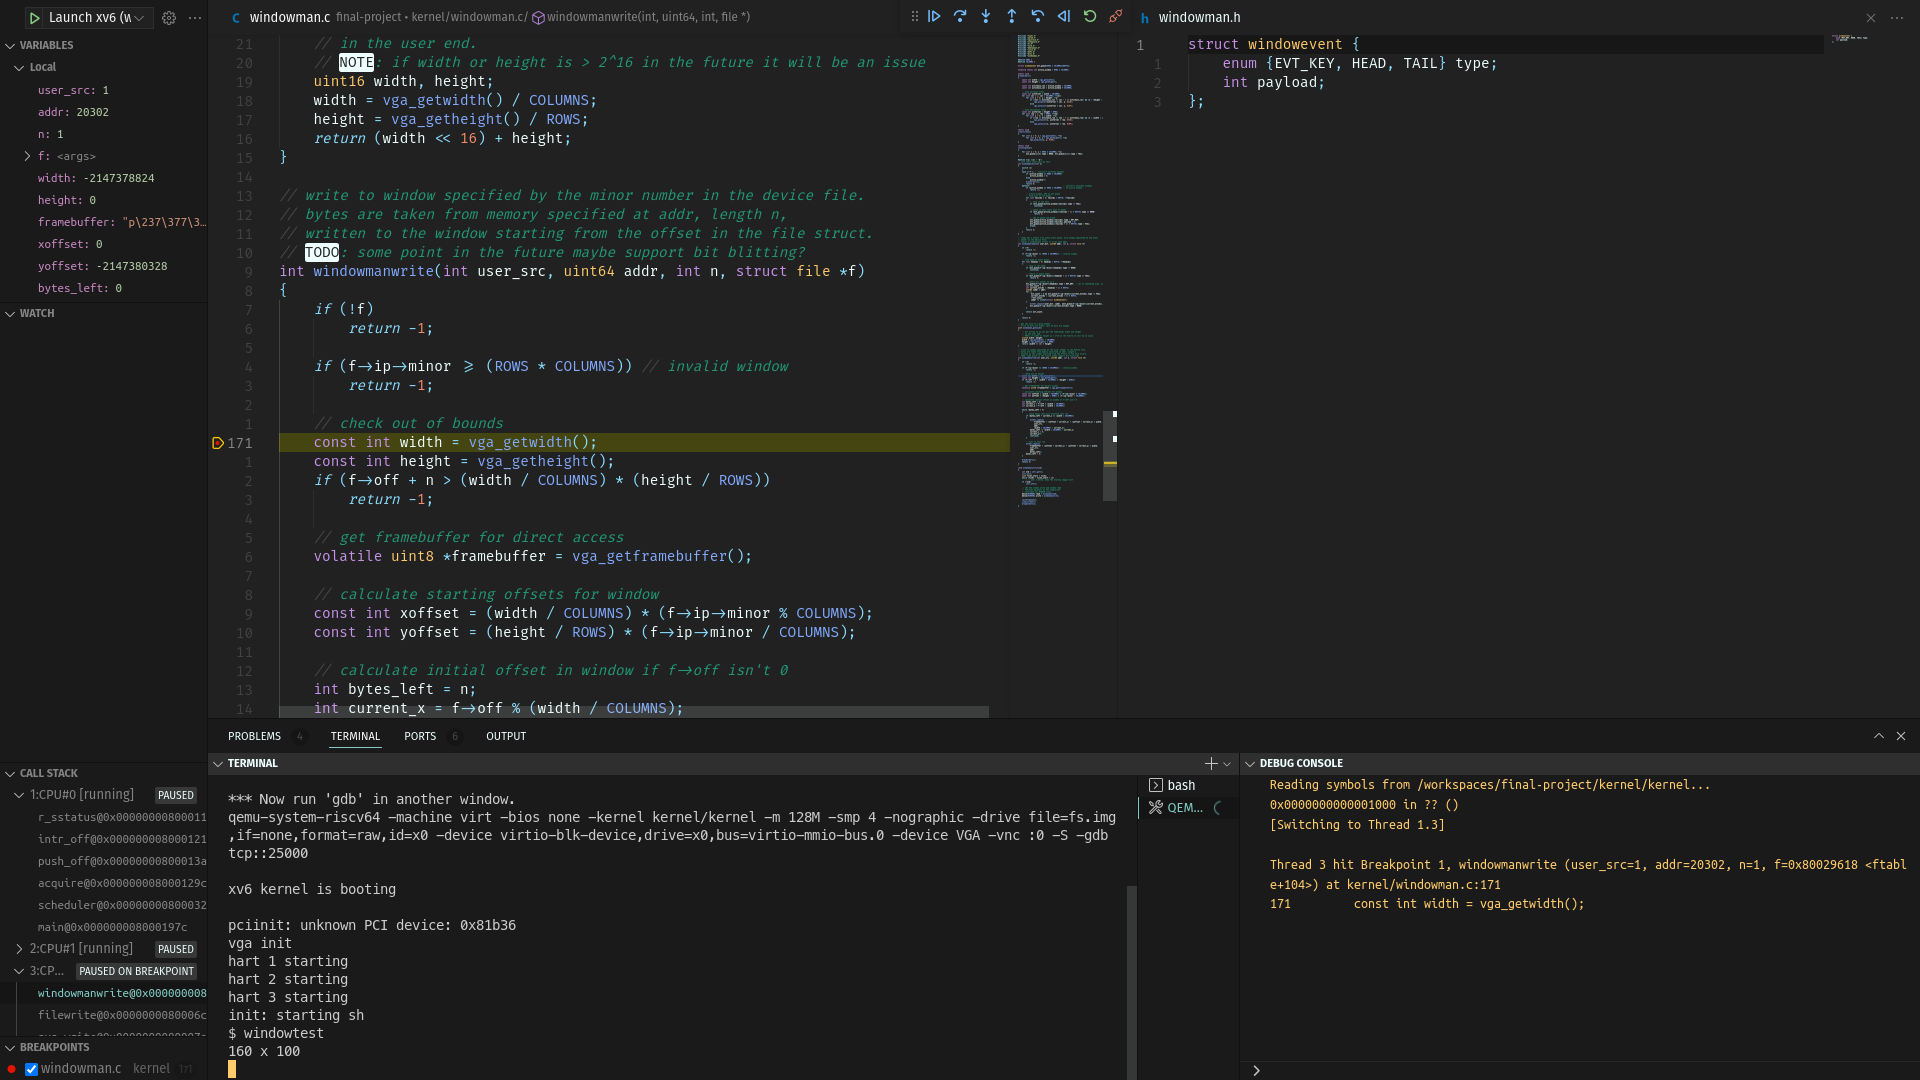
\includegraphics[width=15cm]{Screenshot from 2022-04-26 13-05-47.png}
    \caption{Visual Studio Code Debugging}
    \label{figure:2}
\end{figure}

